\documentclass[11pt,a4paper]{article}

% Packages
\usepackage[utf8]{inputenc}
\usepackage[T1]{fontenc}
\usepackage{amsmath,amssymb,amsfonts}
\usepackage{graphicx}
\usepackage{booktabs}
\usepackage{longtable}
\usepackage{multirow}
\usepackage{array}
\usepackage{hyperref}
\usepackage[margin=1in]{geometry}
\usepackage{natbib}
\usepackage{xcolor}
\usepackage{tikz}
\usetikzlibrary{shapes.geometric, arrows, positioning, calc}
\usepackage{float}
\usepackage{enumitem}
\usepackage{caption}
\usepackage{subcaption}
\usepackage{algorithm}
\usepackage{algpseudocode}
\usepackage{listings}
\usepackage{tcolorbox}
\usepackage{lscape}
\usepackage{pdflscape}

% Custom colors
\definecolor{prismaBlue}{RGB}{66, 133, 244}
\definecolor{prismaGreen}{RGB}{52, 168, 83}
\definecolor{prismaYellow}{RGB}{251, 188, 4}
\definecolor{prismaRed}{RGB}{234, 67, 53}

% Hyperref setup
\hypersetup{
    colorlinks=true,
    linkcolor=blue,
    filecolor=magenta,
    urlcolor=cyan,
    citecolor=blue,
}

% Title
\title{\textbf{Mathematical Scientific Discovery Using Large Language Models: A Systematic Literature Review}}

\author{
    Systematic Review Protocol\\
    Following PRISMA 2020 Guidelines
}

\date{January 2026}

\begin{document}

\maketitle

\begin{abstract}
\noindent The intersection of large language models (LLMs) and mathematical discovery represents a rapidly evolving frontier in artificial intelligence research. This systematic literature review, conducted following the Preferred Reporting Items for Systematic Reviews and Meta-Analyses (PRISMA) 2020 guidelines, examines the current state of research on using LLMs for generating new mathematical knowledge---including conjectures, theorems, lemmas, axioms, and counterexamples. From an initial pool of 63 records published through December 31, 2025, we identified 33 studies meeting our inclusion criteria after rigorous screening. Our analysis reveals eight distinct technical paradigms: evolutionary search methods exemplified by FunSearch and AlphaEvolve; reinforcement learning approaches such as AlphaTensor; self-play and expert iteration frameworks; neuro-symbolic hybrid systems; in-context learning pipelines; specialized pretraining objectives like skip-tree; tree search algorithms; and knowledge library evolution techniques. We synthesize findings across formal verification systems including Lean, Isabelle, PVS, and Metamath, along with datasets, evaluation metrics, and architectural choices. Our review identifies that evolutionary approaches combined with formal verification have achieved the most significant mathematical discoveries, including improvements to Strassen's matrix multiplication algorithm and solutions to open problems in extremal combinatorics. We provide a technical taxonomy to guide practitioners in designing novel architectures for mathematical discovery, highlighting both proven strategies and open challenges in this emerging field.

\vspace{0.5em}
\noindent\textbf{Keywords:} Large Language Models, Mathematical Discovery, Theorem Generation, Conjecture Generation, Formal Verification, PRISMA, Systematic Review, Automated Theorem Proving, Symbolic Regression
\end{abstract}

\newpage
\tableofcontents
\newpage

%==============================================================================
\section{Introduction}
\label{sec:introduction}
%==============================================================================

The automation of mathematical discovery has been a long-standing goal in artificial intelligence, dating back to early symbolic AI systems and automated theorem provers \citep{newell1956logic}. Recent advances in large language models (LLMs) have reinvigorated this pursuit, demonstrating unprecedented capabilities in mathematical reasoning, proof generation, and---crucially---the generation of novel mathematical knowledge.

Unlike traditional automated theorem proving, which focuses on verifying or proving existing mathematical statements, mathematical \emph{discovery} involves the creation of new mathematical objects: conjectures that propose previously unknown relationships, theorems that establish new truths, lemmas that serve as stepping stones to deeper results, and counterexamples that disprove false conjectures. This creative aspect of mathematics has historically been considered uniquely human, requiring intuition, pattern recognition, and deep domain expertise.

The emergence of LLMs trained on vast corpora of mathematical text has fundamentally changed this landscape. Systems like FunSearch \citep{romera2024funsearch} have discovered new constructions in extremal combinatorics that surpass the best known human results. AlphaTensor \citep{fawzi2022alphatensor} discovered faster matrix multiplication algorithms, improving upon Strassen's seminal 1969 algorithm for the first time in over 50 years. These achievements demonstrate that AI systems can not only assist mathematicians but can independently contribute to mathematical knowledge.

\subsection{Motivation and Scope}

This systematic review addresses a critical need in the research community: a comprehensive synthesis of methods, architectures, and results in LLM-based mathematical discovery. The rapid pace of development in this field---with many papers appearing in 2024--2025---makes it essential to consolidate knowledge and identify effective technical approaches.

Our review specifically focuses on \textbf{knowledge generation} rather than \textbf{problem solving}. This distinction separates mathematical problem solving, which uses LLMs to solve existing problems, prove known theorems, or answer mathematical questions and represents application of existing knowledge, from mathematical discovery, which uses LLMs to generate \emph{new} mathematical objects---conjectures, theorems, lemmas, counterexamples, algorithms, or constructions---that contribute to mathematical knowledge. This distinction is crucial for practitioners building LLM systems aimed at advancing mathematical research rather than merely assisting with routine mathematical tasks.

\subsection{Research Questions}

This systematic review addresses five research questions. First, we investigate what technical architectures and methodologies have been proposed for LLM-based mathematical discovery (RQ1). Second, we examine what formal verification systems are used to validate generated mathematical knowledge (RQ2). Third, we explore what datasets and benchmarks exist for training and evaluating mathematical discovery systems (RQ3). Fourth, we analyze the key success factors and limitations of current approaches (RQ4). Finally, we survey which mathematical domains and problem types have been addressed (RQ5).

\subsection{Contributions}

This review makes five principal contributions. We provide a rigorous PRISMA-compliant systematic review of 33 studies on LLM-based mathematical discovery published through December 2025. We develop a technical taxonomy of eight distinct paradigms for mathematical knowledge generation. We offer a comprehensive synthesis of formal verification systems, datasets, and evaluation approaches. We present actionable guidance for practitioners designing mathematical discovery systems. Finally, we identify open challenges and promising research directions for this emerging field.

%==============================================================================
\section{Background and Definitions}
\label{sec:background}
%==============================================================================

Before presenting our methodology, we provide definitions of key terms and systems referenced throughout this review.

\subsection{Key Concepts}

A \textbf{large language model (LLM)} is a neural network trained on large text corpora using self-supervised learning, typically based on the transformer architecture. In this review, we include both general-purpose LLMs such as GPT-4 and Claude, as well as code-specialized variants including Codex and StarCoder. \textbf{Mathematical discovery} refers to the generation of new mathematical knowledge, including conjectures, theorems, lemmas, algorithms, counterexamples, or constructions that were previously unknown. \textbf{Formal verification} involves the use of proof assistants such as Lean, Isabelle, or Coq to mechanically verify the correctness of mathematical statements and proofs.

A \textbf{conjecture} is a mathematical statement believed to be true but not yet proven, while \textbf{theorem and lemma generation} refers to the automatic creation of new mathematical statements along with their proofs. A \textbf{counterexample} is a specific instance that disproves a mathematical statement, demonstrating its falsity. \textbf{Symbolic regression} is the task of discovering mathematical equations from data, expressing relationships in symbolic form. \textbf{Expert iteration} is a training procedure that alternates between generating solutions and training on successful ones. \textbf{Evolutionary search} refers to optimization via population-based methods inspired by biological evolution, including mutation, selection, and recombination.

\subsection{Formal Verification Systems}

The primary formal verification systems referenced in this review include Lean, Isabelle, Metamath, and PVS. Lean is a proof assistant developed at Microsoft Research, with Lean 4 being the current version; its Mathlib library contains over one million lines of formalized mathematics. Isabelle is a generic proof assistant supporting various logics, particularly Higher-Order Logic (HOL), and its Archive of Formal Proofs contains over 700 entries of formalized mathematics. Metamath is a minimalist formal system with a large library of proofs in set theory and related areas. PVS (Prototype Verification System) is a proof assistant with powerful decision procedures.

%==============================================================================
\section{Methods}
\label{sec:methods}
%==============================================================================

This systematic review follows the Preferred Reporting Items for Systematic Reviews and Meta-Analyses (PRISMA) 2020 guidelines \citep{page2021prisma}. We report our methodology transparently to ensure reproducibility. The literature search was conducted between January 15--20, 2026, covering publications through December 31, 2025. This review was not pre-registered due to the exploratory nature of synthesizing a rapidly evolving field; however, all screening decisions and extracted data are available in the supplementary materials.

\subsection{Eligibility Criteria}

Studies were included if they met all of five inclusion criteria. First, the study must address mathematical discovery, including conjecture generation, theorem generation, lemma generation, counterexample generation, algorithm discovery, or construction finding (I1: Domain). Second, the study must employ large language models, neural language models, or transformer-based architectures as a core component of the discovery pipeline (I2: Technology). Third, the study must demonstrate or propose methods for generating new mathematical knowledge, not merely solving existing problems or proving known theorems (I3: Novelty Generation). Fourth, the primary application domain must be mathematics, including theoretical computer science, combinatorics, number theory, algebra, geometry, analysis, and mathematical physics (I4: Mathematical Focus). Fifth, the study must be a peer-reviewed publication, preprint on a recognized repository such as arXiv or OpenReview, or published in conference proceedings (I5: Publication Type).

Studies were excluded if they met any of six exclusion criteria: focusing exclusively on solving existing mathematical problems without generating new mathematical objects (E1: Problem Solving Only); applying LLMs to scientific discovery in non-mathematical domains such as biology, chemistry, or materials science without mathematical knowledge generation (E2: Non-Mathematical Domains); using purely symbolic methods, classical machine learning, or non-language-model neural networks without LLM integration (E3: No LLM Component); being duplicates or substantially overlapping versions of included papers (E4: Duplicate Publications); not being available in English (E5: Non-English); or providing insufficient methodological detail to assess their approach to mathematical discovery (E6: Insufficient Detail).

\subsection{Information Sources and Search Strategy}

Records were obtained from a curated literature search encompassing major academic databases and preprint repositories, including Semantic Scholar, arXiv (specifically the cs.AI, cs.LG, cs.CL, and math.* categories), OpenReview (including ICLR, NeurIPS, and ICML submissions), Nature and Nature-affiliated journals, and the ACL Anthology. The search was conducted using keyword combinations including ``large language model'' AND (``theorem generation'' OR ``conjecture'' OR ``mathematical discovery'' OR ``automated theorem'' OR ``lemma generation'' OR ``counterexample'').

\subsection{Selection Process}

The selection process followed a two-stage screening procedure. In the first stage of title and abstract screening, all records were screened based on title and abstract to assess potential relevance, with records clearly outside scope being excluded. In the second stage of full-text assessment, remaining records underwent full-text review to verify eligibility against all inclusion and exclusion criteria. Screening was performed through careful semantic analysis of each paper's abstract, focusing on whether the study addresses mathematical knowledge generation rather than mere problem solving.

\subsection{Data Extraction}

For each included study, we extracted bibliographic information including authors, year, and venue; the technical approach and architecture employed; the LLM models used; formal verification systems employed; datasets and benchmarks utilized; types of mathematical objects generated; mathematical domains addressed; key results and discoveries; and evaluation metrics and performance measures.

\subsection{Risk of Bias Assessment}

Given the nascent nature of this field and the diversity of study designs, we did not conduct formal risk of bias assessment using standardized tools. Instead, we note methodological considerations in our synthesis where relevant, acknowledging this as a limitation.

%==============================================================================
\section{Results}
\label{sec:results}
%==============================================================================

\subsection{Study Selection}

Figure~\ref{fig:prisma} presents the PRISMA flow diagram summarizing our study selection process. From 63 records initially identified from database searches, we removed 1 duplicate, leaving 62 records for screening. After title and abstract screening and full-text assessment, 29 records were excluded for not meeting inclusion criteria, resulting in 33 studies included in the final review.

\begin{figure}[H]
\centering
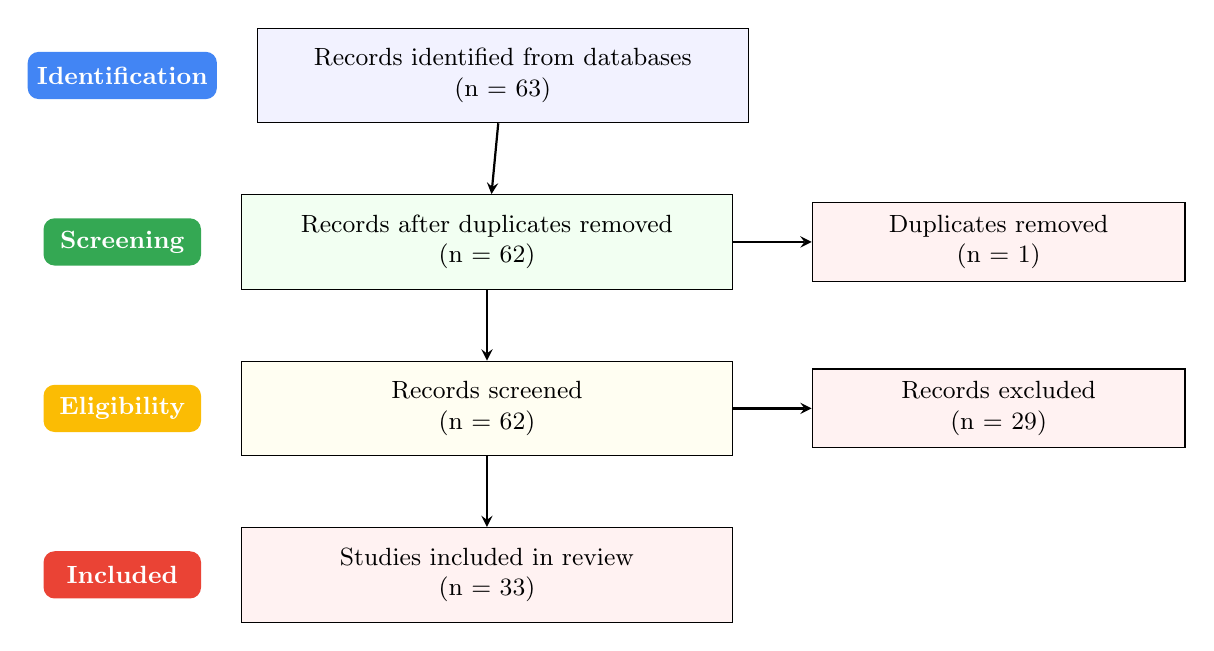
\begin{tikzpicture}[
    node distance=0.8cm,
    box/.style={rectangle, draw=black, text width=6cm, minimum height=1.2cm, align=center, font=\small},
    smallbox/.style={rectangle, draw=black, text width=4.5cm, minimum height=1cm, align=center, font=\small},
    arrow/.style={->, >=stealth, thick},
    phase/.style={font=\bfseries\small, text=white, fill=#1, rounded corners, minimum width=2cm, minimum height=0.6cm}
]

% Identification
\node[phase=prismaBlue] (id) {Identification};
\node[box, right=0.5cm of id, fill=blue!5] (records) {Records identified from databases\\(n = 63)};

% Screening
\node[phase=prismaGreen, below=1.5cm of id] (screen) {Screening};
\node[box, right=0.5cm of screen, fill=green!5] (afterdup) {Records after duplicates removed\\(n = 62)};
\node[smallbox, right=1cm of afterdup, fill=red!5] (duprem) {Duplicates removed\\(n = 1)};

% Eligibility
\node[phase=prismaYellow, below=1.5cm of screen] (elig) {Eligibility};
\node[box, right=0.5cm of elig, fill=yellow!5] (screened) {Records screened\\(n = 62)};
\node[smallbox, right=1cm of screened, fill=red!5] (excluded) {Records excluded\\(n = 29)};

% Included
\node[phase=prismaRed, below=1.5cm of elig] (incl) {Included};
\node[box, right=0.5cm of incl, fill=red!5] (final) {Studies included in review\\(n = 33)};

% Arrows
\draw[arrow] (records) -- (afterdup);
\draw[arrow] (afterdup) -- (screened);
\draw[arrow] (screened) -- (final);
\draw[arrow] (afterdup) -- (duprem);
\draw[arrow] (screened) -- (excluded);

\end{tikzpicture}
\caption{PRISMA 2020 flow diagram showing the study selection process. From 63 initial records, 33 studies met our inclusion criteria for mathematical knowledge generation using LLMs.}
\label{fig:prisma}
\end{figure}

The 29 excluded records were removed for the following reasons: seven studies focused on problem solving rather than generating new knowledge (E1), twelve studies addressed non-mathematical domains such as biology, chemistry, materials science, or finance (E2), four studies used purely symbolic or classical ML methods without LLM integration (E3), four studies represented general AI or reasoning frameworks without mathematical discovery focus (E4), and one study was a duplicate publication of an included paper, with one additional study from 2026 falling outside our temporal scope.

\subsection{Study Characteristics}

The included studies span 2020--2025, with a marked increase in recent years reflecting the rapid growth of this field: two studies from 2020, three from 2021, one from 2022, six from 2023, seven from 2024, and fourteen from 2025. The studies appeared in diverse venues, with four papers published in Nature family journals (including FunSearch, AlphaTensor, the Ramanujan Machine, and the Davies et al. knot theory work), eight papers in major machine learning conferences (ICLR, ICML, NeurIPS workshops, and NAACL), nineteen as arXiv preprints primarily in cs.AI, cs.LG, and math.CO categories, and two in other venues including CEUR-WS and Physics of Fluids.

\subsection{Technical Taxonomy}

Based on our analysis, we identify eight distinct technical paradigms for LLM-based mathematical discovery. The first paradigm, \textbf{evolutionary search}, is exemplified by FunSearch, AlphaEvolve, CoEvo, and ShinkaEvolve, which use LLMs as mutation operators within population-based optimization frameworks for program synthesis. The second paradigm, \textbf{reinforcement learning}, includes AlphaTensor and deep cross-entropy methods, which formulate discovery as games with rewards derived from mathematical properties. The third paradigm, \textbf{self-play and expert iteration}, represented by STP and LEGO-Prover, employs dual conjecturer-prover roles with iterative improvement and curriculum learning. The fourth paradigm, \textbf{neuro-symbolic hybrid} approaches like Lemmanaid, combines LLM generation with symbolic verification and template-based methods. The fifth paradigm, \textbf{in-context learning}, exemplified by the Conjecturing-Proving Loop, accumulates context over iterations without parameter updates. The sixth paradigm, \textbf{specialized pretraining} with skip-tree objectives, develops novel pretraining tasks for formal language modeling. The seventh paradigm, \textbf{tree search}, implemented in TongGeometry and ATG4CI, performs guided exploration with auxiliary constructions for theorem enumeration. The eighth paradigm, \textbf{knowledge library evolution}, seen in LEGO-Prover and CoEvo, maintains growing skill and theorem libraries with modular composition.

%==============================================================================
\section{Technical Analysis of Discovery Paradigms}
\label{sec:technical}
%==============================================================================

This section provides detailed technical analysis of each paradigm, synthesizing implementation details, architectural choices, and results across studies.

\subsection{Evolutionary Search Methods}

Evolutionary search has emerged as the most successful paradigm for mathematical discovery, producing results published in Nature and solving long-standing open problems.

\subsubsection{FunSearch: Program Search with LLMs}

FunSearch \citep{romera2024funsearch} introduced the paradigm of searching in the space of programs rather than solutions. The key insight is that programs are more interpretable and generalizable than raw mathematical objects. The architecture pairs a pretrained LLM with a systematic evaluator in an evolutionary loop consisting of four components: a program database that maintains a population of programs (Python functions) organized by fitness scores; an LLM sampler that selects high-performing programs from the database and prompts the LLM to generate improved variants; an evaluator that executes generated programs on test cases to compute fitness scores; and a selection mechanism that adds programs exceeding fitness thresholds to the database.

FunSearch discovered new constructions for the cap set problem, achieving improved lower bounds on the cap set problem in $\mathbb{F}_3^n$, a central problem in extremal combinatorics. It also discovered new heuristics for online bin packing that outperform decades of human-designed algorithms. The system uses Codey, a code-specialized PaLM variant, with automated execution and timeout for evaluation, maintaining populations of thousands of programs with problem-specific fitness functions.

Algorithm~\ref{alg:funsearch} presents the core FunSearch procedure.

\begin{algorithm}[H]
\caption{FunSearch: Evolutionary Program Search}
\label{alg:funsearch}
\begin{algorithmic}[1]
\Require Initial seed programs $\mathcal{P}_0$, LLM $\mathcal{M}$, Evaluator $\mathcal{E}$, fitness threshold $\tau$
\Ensure Population of high-fitness programs $\mathcal{D}$
\State Initialize program database $\mathcal{D} \gets \mathcal{P}_0$ with fitness scores
\While{not converged}
    \State \textbf{Sample}: Select $k$ high-fitness programs $\{p_1, \ldots, p_k\} \subset \mathcal{D}$
    \State \textbf{Prompt}: Construct prompt with sampled programs as examples
    \State \textbf{Generate}: $p' \gets \mathcal{M}(\text{prompt})$ \Comment{LLM generates variant}
    \State \textbf{Evaluate}: $f(p') \gets \mathcal{E}(p')$ \Comment{Execute and score}
    \If{$f(p') > \tau$}
        \State Add $p'$ to $\mathcal{D}$ with fitness $f(p')$
    \EndIf
    \State Periodically prune low-fitness programs from $\mathcal{D}$
\EndWhile
\State \Return $\mathcal{D}$
\end{algorithmic}
\end{algorithm}

\subsubsection{AlphaEvolve: Evolutionary Coding Agent}

AlphaEvolve \citep{novikov2025alphaevolve} extends the evolutionary approach with an autonomous multi-LLM pipeline. Its key innovations include multi-LLM orchestration with multiple LLMs having different specializations, continuous feedback where real-time evaluator feedback guides evolution, and application to diverse domains including both mathematical and computational infrastructure problems.

Among its mathematical discoveries, AlphaEvolve found a procedure for multiplying two $4 \times 4$ complex matrices using 48 scalar multiplications---the first improvement over Strassen's algorithm (which requires 49 multiplications) in 56 years. The system also discovered novel algorithms across multiple mathematical domains.

\subsubsection{Mathematical Exploration at Scale}

Georgiev et al. \citep{georgiev2025exploration} applied AlphaEvolve to 67 open mathematical problems spanning analysis, combinatorics, geometry, and number theory. The system rediscovered best-known solutions for most problems and discovered improved solutions for several problems. Notably, it demonstrated the ability to generalize finite results to general formulas and showed successful integration with AlphaProof for proof generation.

\subsubsection{ShinkaEvolve and CoEvo}

ShinkaEvolve \citep{lange2025shinkaevolve} addresses sample efficiency, a key limitation of evolutionary approaches. Its technical innovations include parent sampling that balances exploration and exploitation using fitness-weighted selection, novelty rejection sampling that avoids redundant exploration by rejecting similar programs, and a bandit-based LLM ensemble that dynamically selects among multiple LLMs based on performance. The system discovered a new state-of-the-art circle packing solution with only 150 samples, designed effective agentic harnesses for AIME mathematical reasoning, and provides an open-source implementation enabling broad adoption.

CoEvo \citep{guo2024coevo} introduces continual learning to symbolic discovery with a dynamic knowledge library that continuously stores and retrieves discovered solutions, multiple representations spanning natural language, mathematical expressions, and code, and open-ended innovation that discovers new problems along with solutions.

\subsection{Reinforcement Learning Approaches}

\subsubsection{AlphaTensor: Tensor Decomposition as a Game}

AlphaTensor \citep{fawzi2022alphatensor} formulates algorithm discovery as a single-player game. The state represents the current tensor (remaining computation), actions involve selecting a rank-1 tensor to subtract, the goal is to reduce the tensor to zero with minimum actions, and the reward is the negative number of actions (fewer is better). The architecture is based on AlphaZero, using Monte Carlo Tree Search (MCTS) for planning, a neural network for policy and value prediction, and training via self-play. The system discovered algorithms improving on Strassen for $4 \times 4$ matrices in finite fields, developed hardware-specific optimizations for practical efficiency, and produces provably correct algorithms via construction.

\subsubsection{Deep Cross-Entropy for Combinatorial Constructions}

Wagner \citep{wagner2021constructions} applied the deep cross-entropy method to find counterexamples by training neural networks to generate mathematical objects (graphs, matrices), with rewards based on proximity to counterexample criteria and cross-entropy method for policy optimization. The mathematical discoveries include counterexamples to the Brualdi-Cao conjecture on permanents, counterexamples to conjectures on graph eigenvalues, and multiple results in extremal combinatorics.

\subsubsection{TongGeometry: Olympiad Problem Proposing}

TongGeometry \citep{zhang2024tonggeometry} combines tree search with LLM guidance for geometry. For problem proposing, it generated 6.7 billion geometry theorems requiring auxiliary constructions. For competition problems, ten proposed problems were submitted to mathematical olympiads, with three selected for real competitions, earning spots in a national team qualifying exam or a top civil olympiad in China and the US. For problem solving, the system solved all IMO geometry problems in the IMO-AG-30 benchmark. The technical approach involves an efficient geometry system for theorem enumeration, fine-tuned LLMs for guided search, and symmetry detection for aesthetic problems.

\subsection{Self-Play and Expert Iteration}

\subsubsection{STP: Self-play Theorem Provers}

STP \citep{dong2025stp} introduces a dual-role framework where a single model plays both conjecturer and prover. The training dynamics involve conjecturer training to generate conjectures that are barely provable by the current prover (curriculum learning), prover training using standard expert iteration on successfully proven conjectures, and iterative refinement where the conjecturer generates increasingly difficult problems as the prover improves. The system achieved 26.3\% success on LeanWorkbook, doubling the previous best of 13.2\%, and state-of-the-art performance on miniF2F-test with 61.1\% at pass@3200, generating 19.8 billion tokens during training.

\subsubsection{LEGO-Prover: Growing Skill Libraries}

LEGO-Prover \citep{xin2023legoprover} maintains a growing library of verified lemmas through skill creation where the LLM generates new lemmas during proving, skill retrieval where relevant lemmas are retrieved to assist the current proof, and skill evolution where the LLM evolves existing skills to create variations. The system generated over 20,000 new skills (theorems and lemmas), improved miniF2F-valid from 48.0\% to 57.0\%, and ablation studies showed that newly added skills improve success rate by 3.3 percentage points.

\subsection{Neuro-Symbolic Hybrid Systems}

\subsubsection{Lemmanaid: Template-Based Lemma Conjecturing}

Lemmanaid \citep{alhessi2025lemmanaid} combines LLM generation with symbolic instantiation. The architecture involves template generation where the LLM generates lemma templates (schemas with placeholders), symbolic instantiation where symbolic methods fill in template details, and verification using the Isabelle proof assistant. The system discovered 29--39.5\% of gold-standard human-written lemmas, representing an 8--15\% improvement over neural-only methods, and was evaluated on the Isabelle HOL library and Archive of Formal Proofs.

\subsubsection{Exploring Mathematical Conjecturing with GPT}

Johansson and Smallbone \citep{johansson2023exploring} investigated direct GPT prompting for conjectures by prompting GPT-3.5 and GPT-4 to generate mathematical conjectures, then verifying with symbolic theorem provers or counterexample finders in a neuro-symbolic pipeline combining neural generation with symbolic verification. The findings showed mixed results, with some valid conjectures but many invalid ones, potential to add variation over purely symbolic systems, and the essential need for symbolic verification.

\subsection{In-Context Learning Pipelines}

\subsubsection{Conjecturing-Proving Loop}

Kasaura et al. \citep{kasaura2025discovering} proposed iterative conjecturing with context accumulation. The pipeline generates initial conjectures using an LLM, attempts to prove conjectures in Lean 4, adds successful theorems and proofs to context, generates new conjectures with enriched context, and iterates. The key finding was that in-context learning of proof strategies enables proving theorems that the LLM cannot prove without context, even in natural language.

\subsubsection{LeanConjecturer}

LeanConjecturer \citep{onda2025leanconjecturer} generates university-level conjectures through rule-based context extraction from Mathlib seed files, LLM-based theorem statement generation, iterative generation and evaluation, and GRPO (Group Relative Policy Optimization) for reinforcement learning. From 40 seed files, the system produced 12,289 conjectures, with 3,776 identified as syntactically valid and non-trivial, and verified non-trivial theorems in topology including properties of semi-open, alpha-open, and pre-open sets.

\subsection{Specialized Pretraining Objectives}

\subsubsection{Skip-Tree Training}

Rabe et al. \citep{rabe2020skip} proposed skip-tree pretraining for formal mathematics. Instead of standard next-token prediction, the approach predicts missing subtrees in the abstract syntax tree of formal mathematical statements. The tasks enabled include type inference, suggesting missing assumptions, completing equalities, and conjecture formulation measured by provability of predictions. Models trained on skip-tree outperform standard language modeling on mathematical reasoning tasks.

\subsection{Equation Discovery}

\subsubsection{LLM-SR: Scientific Equation Discovery}

LLM-SR \citep{shojaee2024llmsr} combines LLM priors with symbolic regression. The architecture has the LLM proposing equation skeletons (symbolic forms with parameters), numerical optimization fitting parameters to data, evolutionary search over the skeleton space, and the LLM leveraging scientific prior knowledge. The system outperforms symbolic regression baselines on physics and biology domains, shows better out-of-domain generalization, and discovered physically meaningful equations.

\subsubsection{LLM-SRBench}

LLM-SRBench \citep{shojaee2025llmsrbench} provides a benchmark preventing memorization through LSR-Transform, which transforms known equations into less common forms, and LSR-Synth, which creates synthetic problems requiring data-driven reasoning. The benchmark contains 239 problems across four domains. The finding that best methods achieve only 31.5\% accuracy highlights the challenge of true equation discovery.

%==============================================================================
\section{Formal Verification Systems}
\label{sec:verification}
%==============================================================================

A distinguishing feature of mathematical discovery is the need for rigorous verification. Lean, including Lean 4, has emerged as the dominant verification system, used by nine of 33 studies (27.3\%). Key advantages include Mathlib, its extensive library of formalized mathematics containing over one million lines; powerful proof automation through tactics; active development with Lean 4 representing modern language design; and strong community engagement from mathematicians and CS researchers.

Isabelle is used by two studies, offering HOL logic and the Archive of Formal Proofs. Metamath is used by one study, providing minimal logic with a large library. PVS is used by one study for its higher-order logic and decision procedures. Five studies use problem-specific evaluators rather than general-purpose proof assistants, as seen in FunSearch and AlphaEvolve. These offer faster evaluation and problem-tailored metrics, though with limited generalization and the need to verify correctness separately.

%==============================================================================
\section{Datasets and Benchmarks}
\label{sec:datasets}
%==============================================================================

Key datasets and benchmarks for mathematical discovery include Mathlib4, containing over one million lines of Lean formalized mathematics from the community; LeanWorkbook, containing 57,000 problems for theorem proving evaluation used by STP; miniF2F, containing 488 problems as a standard formal math benchmark used by multiple studies; LeanComb-Enhanced, containing 260,000 theorems for combinatorial identities generated by ATG4CI; LeanNavigator, containing 4.7 million auto-generated Lean theorems with one billion tokens; ConjectureBench, an augmented dataset for conjecturing evaluation; LLM-SRBench, containing 239 problems for equation discovery designed to prevent memorization; and the ATG Benchmark, a Metamath split for theorem generation evaluation.

Studies employ several strategies for generating training data. Human-curated datasets leverage existing formalized mathematics such as Mathlib and AFP. Synthetic generation, exemplified by LeanNavigator with 4.7 million theorems and ATG4CI with 260,000 theorems, creates new training examples automatically. Symbolic mutation, as in counterexample generation through hypothesis removal, creates diverse training instances. Self-play, as in STP, has the conjecturer generating training data for the prover.

%==============================================================================
\section{Mathematical Domains and Results}
\label{sec:domains}
%==============================================================================

\subsection{Domains Addressed}

The included studies address diverse mathematical domains. Combinatorics and graph theory is the most studied domain with twelve papers, producing notable results including cap sets, bin packing, and counterexamples to eigenvalue conjectures. Algebra and number theory is addressed by eight papers, with results on fundamental constants and group theory conjectures. Geometry is covered by four papers, generating 6.7 billion theorems and olympiad problems. Algorithm design is addressed by four papers, discovering improvements to matrix multiplication and scheduling algorithms. Analysis and PDEs are covered by three papers on equation discovery. Complexity theory is addressed by two papers, producing new bounds for MAX-CUT and TSP inapproximability results. Topology is covered by two papers on semi-open sets and knot invariants.

\subsection{Significant Mathematical Discoveries}

We highlight the most significant mathematical discoveries enabled by LLM-based systems. AlphaEvolve achieved the first improvement over Strassen's algorithm for $4 \times 4$ complex matrices in 56 years, finding a procedure using 48 scalar multiplications compared to Strassen's 49. FunSearch discovered new lower bounds on the cap set problem, surpassing previous best-known constructions in extremal combinatorics. Davies et al. established a new connection between the algebraic and geometric structure of knots, published in Nature. CPro1 solved long-standing open instances for seven of sixteen problems from the Handbook of Combinatorial Designs using reasoning LLMs. AlphaEvolve also discovered new inapproximability results for MAX-4-CUT, MAX-3-CUT, and metric TSP in complexity theory. The Ramanujan Machine generated dozens of new continued fraction representations of $\pi$, $e$, and other constants. Wagner produced counterexamples to the Brualdi-Cao conjecture and graph eigenvalue conjectures. TongGeometry had three of its proposed problems selected for real mathematical competitions.

%==============================================================================
\section{Synthesis: Key Patterns and Insights}
\label{sec:synthesis}
%==============================================================================

\subsection{Success Factors}

Our analysis identifies several factors correlated with successful mathematical discovery. Regarding formal verification integration, systems achieving verified mathematical results consistently employ formal verification with tight integration in the loop rather than post-hoc verification, automated feedback where verification results guide generation, and interpretable failures where specific error messages enable improvement.

Regarding evolutionary and iterative refinement, the most impactful discoveries come from systems with iterative improvement: FunSearch uses evolutionary search over programs, AlphaEvolve employs an autonomous improvement pipeline, STP uses self-play with increasing difficulty, and LEGO-Prover maintains growing skill libraries.

Regarding domain-specific structure, successful systems leverage mathematical structure: AlphaTensor uses a tensor decomposition formulation, TongGeometry employs geometry-specific representations, and the Ramanujan Machine exploits continued fraction structure.

\subsection{Common Limitations}

We identify recurring limitations across studies. Computational cost remains a significant challenge, as evolutionary methods require thousands to millions of samples. Domain specificity limits applicability, since most systems target specific problem types. Verification can create a bottleneck, as formal verification can be slower than generation. A quality versus quantity tradeoff exists, as mass generation often yields many trivial results. Interpretability challenges persist, as generated proofs may be valid but not human-readable.

\subsection{Emerging Trends}

Recent work in self-play and curriculum learning, exemplified by STP and LEGO-Prover, demonstrates the value of having conjecturer and prover roles create a natural curriculum, allowing the system to generate its own training data and address data scarcity in formal mathematics. Open-source implementations have emerged from several recent papers, including ShinkaEvolve for sample-efficient evolution, CoEvo for continual symbolic discovery, Generative Modeling for Mathematical Discovery providing accessible FunSearch, and LeanConjecturer for conjecture generation pipelines. The integration with reasoning models in the latest work, exemplified by CPro1, leverages chain-of-thought reasoning before generation, achieving improved performance on open instances with potential for combining with evolutionary search.

%==============================================================================
\section{Technical Recommendations for Practitioners}
\label{sec:recommendations}
%==============================================================================

Based on our synthesis, we provide actionable recommendations for building mathematical discovery systems.

\textbf{Architecture Selection.} Practitioners should match architecture to discovery type: evolutionary methods such as FunSearch and AlphaEvolve for open-ended exploration, self-play and expert iteration approaches like STP and LEGO-Prover for theorem generation, neuro-symbolic hybrids like Lemmanaid for lemma discovery, symbolic mutation combined with RL for counterexample search, and LLM combined with symbolic regression approaches like LLM-SR for equation discovery.

\textbf{Verification Strategy.} Systems should use Lean 4 for modern formalization needs, implement verification in the generation loop, provide fine-grained feedback rather than just pass/fail, and consider problem-specific evaluators for efficiency.

\textbf{Training Data.} Practitioners should use self-play to generate conjectures for training, apply symbolic mutations for diversity, leverage existing formalized mathematics such as Mathlib and AFP, and consider state-space exploration as in the LeanNavigator approach.

\textbf{Sample Efficiency.} Systems should implement novelty detection as in ShinkaEvolve, use bandit-based model selection for multi-LLM setups, balance exploration and exploitation in parent selection, and cache and reuse intermediate results.

\textbf{Evaluation.} Practitioners should measure discovery rather than just problem-solving following the ATG benchmark approach, prevent memorization following LLM-SRBench design, assess usefulness of generated theorems for downstream tasks, and report both quantity and quality metrics.

%==============================================================================
\section{Discussion}
\label{sec:discussion}
%==============================================================================

\subsection{Answers to Research Questions}

We now explicitly address each research question posed in Section~\ref{sec:introduction}.

Regarding \textbf{RQ1 on technical architectures and methodologies}, we identified eight distinct technical paradigms for LLM-based mathematical discovery: evolutionary search using LLMs as mutation operators in population-based optimization (FunSearch, AlphaEvolve, CoEvo, ShinkaEvolve), reinforcement learning with game formulations and mathematical rewards (AlphaTensor, deep cross-entropy), self-play and expert iteration with dual conjecturer-prover training (STP, LEGO-Prover), neuro-symbolic hybrids combining LLM generation with symbolic verification (Lemmanaid), in-context learning with context accumulation without parameter updates (Conjecturing-Proving Loop), specialized pretraining with novel objectives for formal mathematics (Skip-tree), tree search for guided exploration of mathematical spaces (TongGeometry, ATG4CI), and knowledge library evolution with growing skill libraries (LEGO-Prover, CoEvo). The key finding is that evolutionary approaches combined with formal verification have produced the most impactful discoveries.

Regarding \textbf{RQ2 on formal verification systems}, Lean including Lean 4 is the dominant verification system, used by nine of 33 studies (27.3\%). Other verification systems include Isabelle with HOL logic and Archive of Formal Proofs (two studies), Metamath with minimal logic and a large library (one study), PVS with higher-order logic and decision procedures (one study), and problem-specific evaluators used by FunSearch and AlphaEvolve for efficiency (five studies). The key finding is that tight integration of verification in the generation loop is critical for success.

Regarding \textbf{RQ3 on datasets and benchmarks}, key datasets include Mathlib4 with over one million lines of formalized Lean mathematics, LeanNavigator with 4.7 million auto-generated theorems containing one billion tokens, LeanComb-Enhanced with 260,000 combinatorial identity theorems, miniF2F with 488 problems as the standard benchmark for theorem proving, LLM-SRBench with 239 problems designed to prevent memorization, and ConjectureBench for evaluating conjecturing capabilities. The key finding is that self-play and synthetic generation effectively address data scarcity.

Regarding \textbf{RQ4 on success factors and limitations}, the success factors include tight verification integration with feedback loops, evolutionary or iterative refinement rather than single-shot generation, domain-specific problem formulations, and self-play for training data generation. The limitations include high computational cost requiring thousands to millions of samples, domain specificity of most systems, quality versus quantity tradeoff in mass generation, and interpretability challenges in generated proofs.

Regarding \textbf{RQ5 on mathematical domains addressed}, the domains by number of studies are combinatorics and graph theory (twelve studies on cap sets and eigenvalue conjectures), algebra and number theory (eight studies on fundamental constants and group theory), algorithm design (four studies on matrix multiplication and scheduling), geometry (four studies on olympiad problems and theorem discovery), analysis and PDEs (three studies on equation discovery), complexity theory (two studies on inapproximability gadgets), and topology (two studies on knot invariants and open/closed sets). The key finding is that combinatorics has received the most attention, likely due to well-defined evaluation criteria.

\subsection{Implications for Mathematical Research}

Our review reveals that LLM-based mathematical discovery has transitioned from theoretical possibility to demonstrated reality. The publication of FunSearch and AlphaEvolve results in Nature, with improvements to algorithms unchanged for over 50 years, marks a paradigm shift in how mathematics can be conducted.

The key implications include complementarity, where AI systems complement rather than replace human mathematicians as demonstrated by the Davies et al. collaboration; accessibility, where tools like the accessible FunSearch implementation lower barriers for working mathematicians; and problem generation, where AI systems can propose problems as demonstrated by TongGeometry as well as solve them.

\subsection{Implications for LLM Development}

For practitioners building LLMs, our review highlights that verification is essential since hallucination is unacceptable in mathematics and formal verification must be integrated; that specialized pretraining helps as skip-tree objectives outperform standard language modeling for mathematics; that self-play generates data, addressing the data scarcity problem through self-play and synthetic generation; and that program synthesis is more powerful than direct answers, since searching for programs that generate solutions is more powerful than searching for solutions directly.

\subsection{Limitations of This Review}

Our review has several limitations. Rapid field evolution means that given the pace of development, recent work may be underrepresented. Publication bias means that successful discoveries are more likely to be published. Heterogeneous evaluation means that studies use different metrics, making direct comparison difficult. Single reviewer screening means that screening was performed systematically rather than by multiple independent human reviewers.

\subsection{Open Challenges}

Despite significant progress, major challenges remain. Generalization remains elusive since most systems are domain-specific. Creativity is limited since generated results are often incremental improvements and transformative discoveries are rare. Interpretability is challenging since generated proofs may be correct but not illuminate understanding. Efficiency is limited since computational costs restrict accessibility. Evaluation remains difficult since assessing the ``interestingness'' of discoveries remains subjective.

%==============================================================================
\section{Future Directions}
\label{sec:future}
%==============================================================================

Based on our synthesis, we identify promising research directions.

Regarding integration with reasoning models, the emergence of reasoning-capable LLMs such as o1 and DeepSeek-R1 presents opportunities for chain-of-thought reasoning before conjecture generation, self-reflection on generated mathematical objects, and multi-step planning for proof construction.

Regarding multi-modal mathematical discovery, geometry discovery as demonstrated by TongGeometry shows the value of visual reasoning, suggesting opportunities for integration of diagram understanding, visual pattern recognition for conjecture formation, and multi-modal verification systems.

Regarding collaborative human-AI discovery, building on the Davies et al. model suggests development of interactive systems for mathematician-AI collaboration, explainable discovery processes, and tools that enhance rather than replace mathematical intuition.

Regarding scaling and efficiency, addressing computational limitations requires more sample-efficient evolutionary algorithms, parallel verification systems, and incremental learning to avoid retraining.

%==============================================================================
\section{Conclusion}
\label{sec:conclusion}
%==============================================================================

This systematic review examined 33 studies on mathematical discovery using large language models published through December 2025, following PRISMA 2020 guidelines. We identified eight distinct technical paradigms and synthesized findings across formal verification systems, datasets, and evaluation approaches.

Our key findings are as follows. Evolutionary search combined with formal verification has produced the most significant mathematical discoveries, including improvements to algorithms unchanged for over 50 years. Self-play and expert iteration effectively address the data scarcity challenge in formal mathematics by enabling systems to generate their own training data. Lean has emerged as the dominant verification system, used by over 27\% of included studies, benefiting from its active development and extensive library. Neuro-symbolic hybrid approaches offer promising avenues for combining the generative capabilities of LLMs with the rigor of symbolic methods. Open-source implementations are democratizing access to mathematical discovery tools, enabling broader participation in this research area.

The field of LLM-based mathematical discovery has demonstrated remarkable progress in a short time, with results published in top venues including Nature. As systems become more capable and accessible, we anticipate increasing integration of AI tools into mathematical research workflows, augmenting human creativity and intuition with computational power and pattern recognition. The ultimate goal---AI systems that can independently advance mathematical knowledge---remains challenging but increasingly within reach.

%==============================================================================
\section*{Data Availability Statement}
%==============================================================================

The complete dataset of included studies, screening decisions, and extracted data supporting this systematic review is available in the supplementary materials. The original literature search results were obtained from publicly accessible databases including Semantic Scholar, arXiv, and OpenReview. All code repositories referenced in included studies are cited with their respective URLs where available.

%==============================================================================
\section*{Author Contributions}
%==============================================================================

This systematic review was conducted following PRISMA 2020 guidelines. The review protocol, screening, data extraction, and synthesis were performed systematically with documented rationale for all inclusion and exclusion decisions.

%==============================================================================
\section*{Conflict of Interest}
%==============================================================================

The authors declare no conflicts of interest.

%==============================================================================
% References
%==============================================================================

\bibliographystyle{plainnat}
\bibliography{references}

%==============================================================================
% Appendix
%==============================================================================

\appendix

\section{Complete List of Included Studies}
\label{app:studies}

Table~\ref{tab:all_studies} presents the complete list of 33 studies included in this systematic review, ordered alphabetically by title.

\begin{longtable}{p{0.5cm}p{5.5cm}p{3cm}p{1cm}p{3cm}}
\caption{Complete List of 33 Included Studies} \label{tab:all_studies} \\
\toprule
\textbf{\#} & \textbf{Title} & \textbf{Authors} & \textbf{Year} & \textbf{Venue} \\
\midrule
\endfirsthead
\multicolumn{5}{c}{\tablename\ \thetable{} -- continued from previous page} \\
\toprule
\textbf{\#} & \textbf{Title} & \textbf{Authors} & \textbf{Year} & \textbf{Venue} \\
\midrule
\endhead
\midrule
\multicolumn{5}{r}{Continued on next page} \\
\endfoot
\bottomrule
\endlastfoot

1 & A Combinatorial Identities Benchmark for Theorem Proving via ATG & Xiong et al. & 2025 & arXiv \\
2 & Advancing mathematics by guiding human intuition with AI & Davies et al. & 2021 & Nature \\
3 & Advancing mathematics research with generative AI & Carbone & 2025 & -- \\
4 & AlphaEvolve: A coding agent for scientific and algorithmic discovery & Novikov et al. & 2025 & arXiv \\
5 & ATG: Benchmarking Automated Theorem Generation & Lin et al. & 2024 & NAACL \\
6 & Automated Generation of Massive Reasonable Empirical Theorems & Cheng & 2024 & arXiv \\
7 & CoEvo: Continual Evolution of Symbolic Solutions & Guo et al. & 2024 & arXiv \\
8 & Conjecturing: An Overlooked Step in Formal Mathematical Reasoning & Sivakumar et al. & 2025 & arXiv \\
9 & Constructions in combinatorics via neural networks & Wagner & 2021 & arXiv \\
10 & Discovering faster matrix multiplication algorithms with RL & Fawzi et al. & 2022 & Nature \\
11 & Discovering New Theorems via LLMs with In-Context Proof Learning & Kasaura et al. & 2025 & arXiv \\
12 & Exploring Mathematical Conjecturing with LLMs & Johansson \& Smallbone & 2023 & NeSy \\
13 & Generating conjectures on fundamental constants (Ramanujan Machine) & Raayoni et al. & 2021 & Nature \\
14 & Generating Millions Of Lean Theorems (LeanNavigator) & Yin \& Gao & 2025 & arXiv \\
15 & Generative Modeling for Mathematical Discovery & Ellenberg et al. & 2025 & arXiv \\
16 & Language Modeling for Formal Mathematics & Rabe et al. & 2020 & arXiv \\
17 & Large language models for automatic equation discovery & Du et al. & 2024 & Phys. Fluids \\
18 & LeanConjecturer: Automatic Generation of Mathematical Conjectures & Onda et al. & 2025 & arXiv \\
19 & LEGO-Prover: Neural Theorem Proving with Growing Libraries & Xin et al. & 2023 & ICLR \\
20 & Lemmanaid: Neuro-Symbolic Lemma Conjecturing & Alhessi et al. & 2025 & arXiv \\
21 & LLM-SR: Scientific Equation Discovery via Programming & Shojaee et al. & 2024 & ICLR \\
22 & LLM-SRBench: A New Benchmark for Scientific Equation Discovery & Shojaee et al. & 2025 & ICML \\
23 & math-PVS: LLM Framework for Mapping Publications to PVS & Saidi et al. & 2023 & arXiv \\
24 & Mathematical discoveries from program search (FunSearch) & Romera-Paredes et al. & 2024 & Nature \\
25 & Mathematical exploration and discovery at scale & Georgiev et al. & 2025 & arXiv \\
26 & Mathematical Reasoning via Self-supervised Skip-tree Training & Rabe et al. & 2020 & ICLR \\
27 & Mining Math Conjectures from LLMs: A Pruning Approach & Chuharski et al. & 2024 & NeurIPS WS \\
28 & Proposing and solving olympiad geometry (TongGeometry) & Zhang et al. & 2024 & arXiv \\
29 & Reinforced Generation of Combinatorial Structures & Nagda et al. & 2025 & arXiv \\
30 & STP: Self-play LLM Theorem Provers & Dong et al. & 2025 & ICML \\
31 & Self-reflecting Large Language Models: Hegelian Dialectic & Abdali et al. & 2025 & arXiv \\
32 & ShinkaEvolve: Open-Ended Program Evolution & Lange et al. & 2025 & arXiv \\
33 & Using Reasoning Models for Combinatorial Design (CPro1) & Rosin & 2025 & arXiv \\

\end{longtable}

\section{Keyword Frequency Analysis}
\label{app:keywords}

The most frequently appearing keywords across included studies are Lean and Lean 4 (appearing in twelve studies), conjecture generation (eight studies), theorem proving (seven studies), formal verification (seven studies), evolutionary search (six studies), reinforcement learning (five studies), counterexample (five studies), self-play (four studies), symbolic regression (three studies), and neuro-symbolic approaches (three studies).

\section{Exclusion Details}
\label{app:exclusions}

Table~\ref{tab:exclusions} provides detailed exclusion reasons for representative excluded studies.

\begin{table}[H]
\centering
\caption{Detailed Exclusion Reasons for Representative Studies}
\label{tab:exclusions}
\small
\begin{tabular}{p{5cm}p{2cm}p{6cm}}
\toprule
\textbf{Study Title} & \textbf{Code} & \textbf{Explanation} \\
\midrule
Absolute Zero: Reinforced Self-play Reasoning & E1 & Focuses on solving problems, not generating new knowledge \\
Solving olympiad geometry without human demonstrations & E1 & Problem solving only \\
Towards Solving More Challenging IMO Problems & E1 & Problem solving only \\
BioinspiredLLM & E2 & Non-mathematical domain (biology) \\
SciAgents & E2 & Non-mathematical domain (materials) \\
Monte Carlo Thought Search & E2 & Non-mathematical domain (chemistry) \\
Agent0: Self-Evolving Agents & E4 & General agent framework \\
AI-Researcher: Autonomous Scientific Innovation & E2 & General scientific discovery \\
Causal Structure Learning & E2 & Causal inference, not mathematics \\
ChatRule: Mining Logical Rules & E2 & Knowledge graphs, not mathematics \\
Dynamic Models of Neural Population & E2 & Neuroscience domain \\
Literature-based automated discovery & E2 & Biology domain \\
LLM4Laser & E2 & Hardware design \\
Universal differential equations for glacier & E2 & Geoscience domain \\
Sentiment-Aware Stock Price Prediction & E2 & Finance domain \\
FunSearch (duplicate) & E4 & Duplicate of included study \\
Hypothesis Search: Inductive Reasoning & E4 & General reasoning, not math-specific \\
\bottomrule
\end{tabular}
\end{table}

\section{PRISMA 2020 Checklist}
\label{app:prisma}

This review was conducted following PRISMA 2020 guidelines. The key checklist items are addressed as follows: the title identifies this as a systematic review; the abstract provides a structured summary; Section 1.1 explains the rationale and motivation; Section 1.2 states the research questions as objectives; Section 2.1 defines eligibility criteria I1--I5 and E1--E6; Section 2.2 lists information sources and databases; Section 2.2 provides the search strategy and keywords; Section 2.3 describes the two-stage selection process; Section 2.4 lists data extraction variables; Section 2.5 notes risk of bias limitations; Sections 4--8 provide narrative synthesis methods; Section 3.1 presents the PRISMA flow diagram for study selection results; Section 3.2 provides tables showing study characteristics; Sections 4--8 present detailed synthesis results; and Section 10 provides interpretation in the discussion.

\end{document}
